% !TEX root = ../rapport.tex

\newpage
\section{Idégenerering}
For at sætte den hurtigste omgangstid skal der være en kombination af den rigtig fysiske opsætning af bilen og en microprocessor der fortæller bilen hvordan den skal køre på banen. Det første der blev undersøgt var de fysiske optimeringer der kunne laves på bilen.
\subsection{Hardware}
\begin{itemize}
\item Forøgelse af acceleration og tophastighed
\item Formindskelse af bremselængde
\item Optimering hastighed igennem sving
\end{itemize}
For at optimere ovenstående er der flere ting der kan overvejes, se figur \ref{fig:mindmap1}.

\begin{figure}[ht]
    \centering
    \includegraphics[width=1\textwidth]{kapitler/billeder/Mindmap1.jpg}
    \caption{Idégenerering til optimering af omgangstid}
    \label{fig:mindmap1}
\end{figure}

\subsection{Software}

Udover de fysiske ting i bilen skal bilens omgangstid også optimeres ved hjælp af software.


\newpage

\begin{figure}[ht]
    \centering
    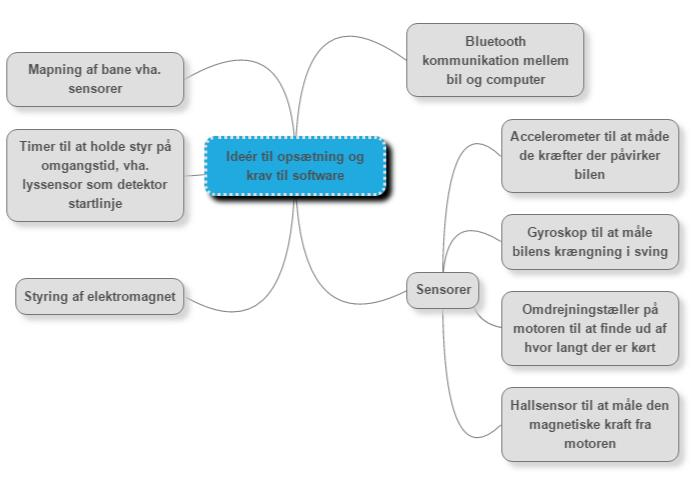
\includegraphics[width=0.8\textwidth]{kapitler/billeder/Mindmap2.jpg}
    \caption{Idégenerering til opsætning af software}
    \label{fig:mindmap2}
\end{figure}


Idéen er ved hjælp af sensorerne skal softwaren kunne mappe den ukendte bane ved at kører et par omgange på den. Når banen er blevet mappet og gemt i bilens hukommelse kan den så sætte en hurtig omgangs tid da den ved hvornår der er et sving hvor der skal bremse og hvor hårdt den kan accelerere de forskellige steder på banen.

Så idéen er at bilen skal optimeres til at køre en så hurtig omgangstid som muligt ved både at optimere det fysiske på bilen, dens hardware og software.
